\documentclass[11pt,letterpaper]{article}
\usepackage[lmargin=1in,rmargin=1in,tmargin=1in,bmargin=1in]{geometry}
\usepackage{../style/homework}
\usepackage{../style/commands}
\setbool{quotetype}{true} % True: Side; False: Under
\setbool{hideans}{false} % Student: True; Instructor: False

% -------------------
% Content
% -------------------
\begin{document}

\homework{8: Due 10/30}{The beauty of mathematics only shows itself to more patient followers.}{Maryam Mirzakhani}

% Problem 1
\problem{10} For each of the following, describe whether the given dependent variable is a function of the independent variable:
	\begin{enumerate}[(a)]
	\item Independent: Number of stains removed by a test detergent. 
		Dependent: Type of detergent used. 
	\item Independent: Time since the song began.
		Dependent: Number of words spoken in the song. 
	\item Independent: Phase of the moon.
		Dependent: Day of the week. 
	\item Independent: Number of days since an account was opened. 
		Dependent: Amount of money in the account. 
	\end{enumerate}



\newpage



% Problem 2
\problem{10} Determine whether the relations $F$ and $G$ shown below are functions. Be sure to fully justify your answer. \pspace
	\hfill
	\begin{minipage}[c]{0.48\textwidth}
	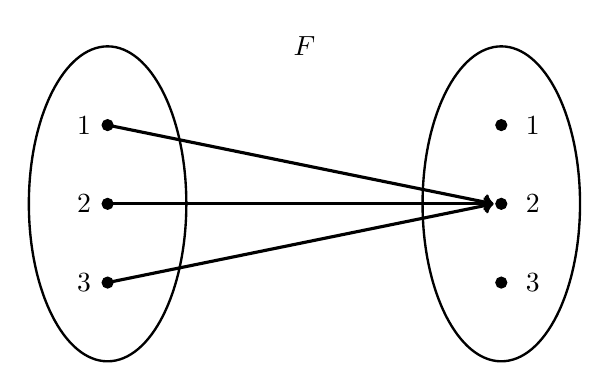
\begin{tikzpicture}
	\node at (2.5,2) {$F$};
	% Ellipses
	\draw[line width=0.03cm] (0,0) circle (1 and 2);
	\draw[line width=0.03cm] (5,0) circle (1 and 2);
	
	% Nodes
	\draw[fill=black] (0,1) circle (0.07);
	\draw[fill=black] (0,0) circle (0.07);
	\draw[fill=black] (0,-1) circle (0.07);
	
	\draw[fill=black] (5,1) circle (0.07);
	\draw[fill=black] (5,0) circle (0.07);
	\draw[fill=black] (5,-1) circle (0.07);
	
	% Arrow
	\draw[line width=0.04cm,->] (0,1) -- (4.9,0);
	\draw[line width=0.04cm,->] (0,0) -- (4.9,0);
	\draw[line width=0.04cm,->] (0,-1) -- (4.9,0);
	
	% Labels
	\node at (-0.3,1) {$1$};
	\node at (-0.3,0) {$2$};
	\node at (-0.3,-1) {$3$};
	
	\node at (5.4,1) {$1$};
	\node at (5.4,0) {$2$};
	\node at (5.4,-1) {$3$};
	\end{tikzpicture}
	\end{minipage}%
	\begin{minipage}[c]{0.40\textwidth}
	\begin{table}[H]
	\centering
	\begin{tabular}{cc}
	$x$ & $G$ \\ \hline
	$1$ & $0$ \\
	$2$ & $2$ \\
	$3$ & $4$ \\
	$4$ & $7$ \\
	$5$ & $0$
	\end{tabular}
	\end{table}
	\end{minipage} \pspace



\newpage



% Problem 3
\problem{10} Determine whether the relations $f(x)= 3x^2 - 4x + 5$ and $g(x, y)= xy^2 - x^2y$ are functions. Be sure to fully justify your answer. Also, find $f(-1)$ and $g(3, -1)$. 


\end{document}